%% ========================================================================
%%							NNLS
%% ========================================================================


\chapter{Neural Networks (NN)}
\label{cha:NN}

In the last chapter of this thesis, a mathematical concept is discussed that has attracted much attention in the recent past, namely neural networks. The area of artificial intelligence (AI) in which neural networks are embedded has been the subject of an intense media hype in recent years. In 2016, for example, a computer program developed by the British company Google DeepMind succeeded for the first time in defeating Lee Sedol of South Korea, considered to be the strongest Go player in the world \cite{wiki_01}. This victory of a machine against a human being is considered to be a milestone in the field of artificial intelligence \cite{LA_Times}. Further successes were also achieved in the area of real-time games at the beginning of 2019. For the first time DeepMind's program called AlphaStar was able to defeat the world's best players in StarCraft which is considered to be one of the most challenging real-time strategy games \cite{AlphaStar}. Also Gartner, a global research and advisory firm, which publishes the well-known but definitely criticisable hype cycle representations considers AI as one of the most important technologies of recent years. In the hype cyle for emerging technologies from 2017 there are 4 out of the 32 listed technologies that can be attributed to the field of AI, such as Deep Learning or Machine Learning \cite{Gartner2017}. Also in the following years 2018 and 2019 technologies that clearly belong to the AI sector were mentioned in the hype cycle 5 and 6 times respectively \cite{Gartner2018}, \cite{Gartner2019}. This trend towards new methods based on neruonal networks can also be seen in other places, such as Kaggle. With more than one million registered users, Kaggle is one of the world's largest platforms for data science competitions and attracts teams from all over the world with prize money in the millions \cite{Kaggle}. It can be observed that, besides gradient boosting, one of the most important concepts with which to win Kaggle competitions is the concept of neural networks in various forms.   

It is therefore clear to see that on the one hand the technology behind AI has enormous potential to solve problems that have so far been assumed to be solved only by humans. On the other hand, it can be assumed that this trend is not just a short-lived phenomenon, but a continuous process leading to business solutions which are based on AI-systems. Therefore, it is even more important to understand the underlying concepts of these technologies and to discuss their applicability in the insurance industry. Whether in the end a completely automated grouping algorithm based on neural networks is possible at all or can be implemented with the available resources remains open. However, the aim is to provide an overview of the basic concepts and to present case studies with insurance cashflows. Since various terms and buzzwords related to artificial intelligence are often used differently in media reports, it is useful to classify some of the most often used terms in order to show their relationship and provide a general framework which is based on \cite{Allaire2018}. 

\begin{figure}
	\centering
	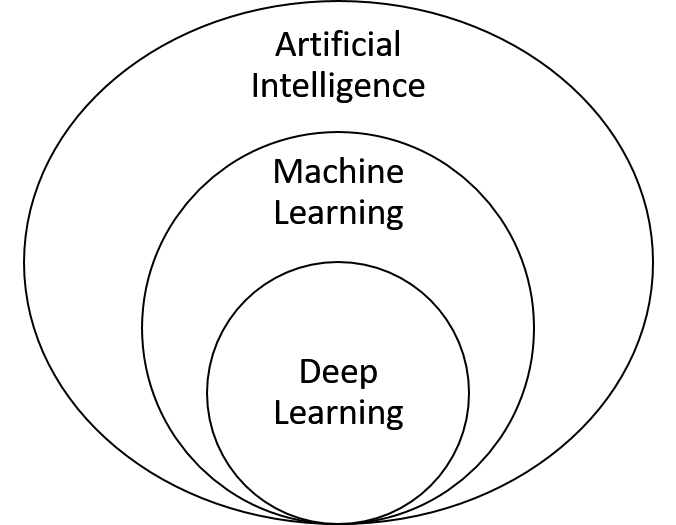
\includegraphics[width=0.5\textwidth]{figures/chapter_NN/framework}
	\caption{Relation of Artificial Intelligence, Machine Learning, and Deep Learning.}
	\label{fig:framework}
\end{figure}

\begin{itemize}
	\item Artificial Intelligence: Artificial Intelligence is a branch of computer science that deals with the programming of intelligent computer systems. Due to a missing definition of the term intelligence the question which types of computer programs are included is not clearly definable. In addition to machine learning and deep learning, there are many other approaches that do not include any kind of learning but are also part of AI. 
	\item Machine Learning: Machine learning arises from this question if it is possible to design a program in such a way that it can learn how to perform a specific task automatically. Given a set of input data and the corresponding results the task is to derive rules. These rules are therefore the output of the machine learning algorithm and can then be used to derive the results for new input data. What all these methods have in common is the fact that they actually try to identify statistical patterns in the data. Thus the aim is to find a meaningful representation of the given data by projections, translations, rotations, nonlinear transformations or any other method and to apply it then to new input data. 	 
	\item Deep Learning: Deep learning, as a sub field of machine learning, focuses on the progressive learning of several levels of abstraction which are increasingly meaningful representations of the data. One can think of the method as a multistage information distillation process where in every single process step a more meaningful representation of the data is obtained. The term deep in deep learning is a reference to the multiple layers which store the abstract representations of the input data in such an algorithm. The number of layers that contribute to a meaningful representation of the data is called depth. Although there is a considerable amount of learning involved, models with several hundred layers are quite common, depending on the type of problem at hand. The concept of the neural network is a reference to the field of neurobiology and the neurons that are connected in different ways in the human brain. Although neuronal networks are not models of the human brain, it is surprising what amazing results can be achieved with such a simple idea and a sufficiently large amount of data.
\end{itemize}
After a brief classification of the terms, the next section describes the basic structure and functionality of neural networks.

\section{Fundamentals of Neural Networks}

In the previous section the functionality of neuronal networks was already described in a rather abstract way as a multi-stage information distillation process. After this high level explanation, the focus is now on pointing out which individual components make up a simple neural network. Figure (\ref{fig:NN_overview}) shows a schematic representation of the individual components required to build a basic neural network. The starting point for the training of any neural network is the input data \texttt{Input X} and the associated outputs \texttt{True targets Y}. These two exogenous quantities must have a standardized numeric form so that the neural network can process them. For example, images of animals can serve as input data and the corresponding target values would then be names of the animals recognizable from the image. Thus, every image which is represented as a number matrix for further processing in the neuronal network is assigned to an animal. In the initial step, the input data is transferred to the first layer. This layer executes a data transformation based on some weights. After the first layer, the transformed output from the current layer servers as input for the next layer which then performs another data transformation based on the weights belonging to this new layer. After the data has passed through the last layer of the model, the transformed data can be used to generate \texttt{Predictions Y'} of the output values. After the first output values have been predicted from the input values, it is necessary to evaluate how well those values match with the actual outputs. For this purpose the true as well as the predicted outputs are fed into a so-called loss function. This function now compares the deviations of the two outputs using a mathematical procedure and returns a loss score.  This loss score is now a measure of how strong the the predicted values \texttt{Y'} deviate from the true values \texttt{Y}. A greater loss score therefore means that there is still a significant deviance between the true and the predicted outputs. 

\begin{figure}
	\centering
	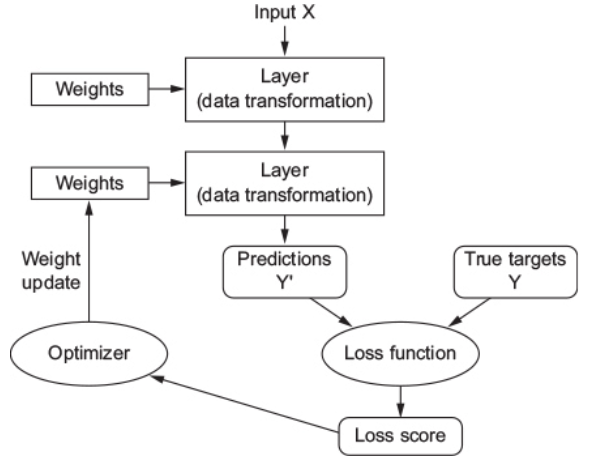
\includegraphics[width=0.65\textwidth]{figures/chapter_NN/NN_overview}
	\caption{Schematic representation of a neural network based on \cite{Allaire2018}}
	\label{fig:NN_overview}
\end{figure}
